\ath{Heiltölubestun} (e. integer programming) hefur margvíslega hagnýtingu í bestun.
Rifjum upp forsendur línulegrar bestunar 
\begin{enumerate}
  \item Engin óvissa í stikum líkansins (e. certainty)
  \item Skorður og markfall línuleg föll
  \item Deilanleiki ákvörðunarbreyta (e. devisibility) 
\end{enumerate}
Ef
\begin{enumerate}
  \item er ekki uppfyllt $\Rightarrow$ \ath{slembin bestun} (e. stochastic programming)
  \item er ekki uppfyllt $\Rightarrow$ \ath{ólínuleg bestun} (e. nonlinear programming)
  \item er ekki uppfyllt $\Rightarrow$ \ath{heiltölubestun} (e. integer programming)
\end{enumerate}

Í mörgum hagnýtum verkefnum er deilanleikaforsendan ógild eða hæpin forsenda. Sem dæmi má nefna bestun á vaktaplani þar sem ákvarðanabreytur svara til fjölda starfsmanna á vakt. Lausnir þar sem fjöldinn er ekki heiltölur hafa enga merkingu, hvernig á að túlka 1.5 starfsmenn?

Ef gildi ákvarðanabreyta í bestu lausn eru nálguð að næstu heiltölu getur nýja lausnin verið umtalsvert lakari en \emph{besta} heiltölulausn eða það sem verra er hún er ekki endilega gjaldgeng.

\begin{samepage}
\begin{daemi}\label{daemi:ip:myndr}Gjaldgenga svæðið afmarkað af skorðum verkefnisins er skyggt og svartir punktar eru gjaldgengar lausnir. Besta lausn línulega bestunarverkefnisins er $(\frac{3}{2},2)$. Aftur á móti eru rúnuðu lausnirnar annaðhvort $(1,2)$ eða $(3,2)$ -- báðar ógjaldgengar. 
\begin{center}
  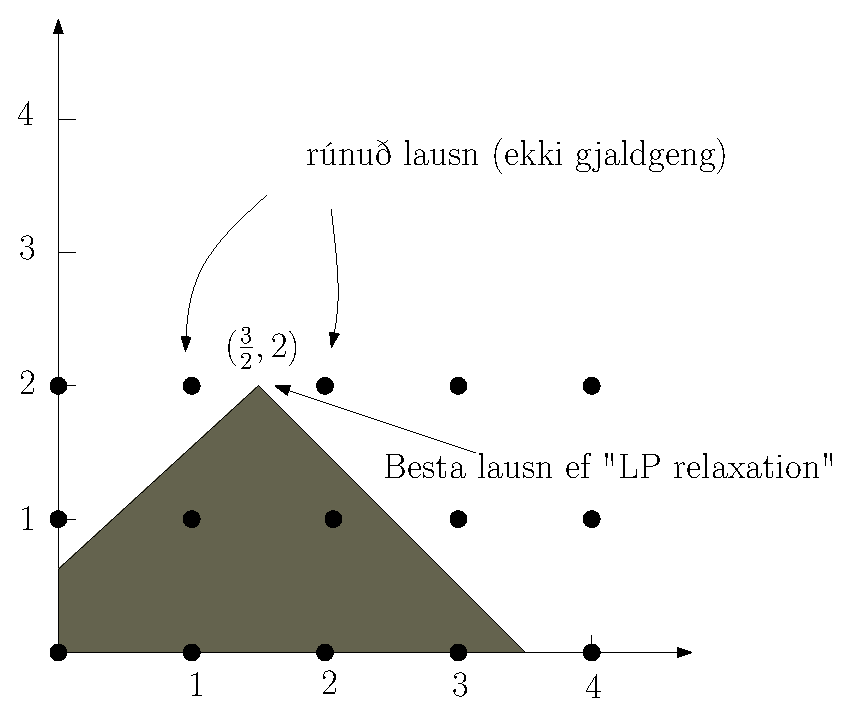
\includegraphics[width=0.7\columnwidth]{figs/relaxation.eps}
\end{center}
\end{daemi}
\end{samepage}

\begin{aths}Ef slakað er á kröfum ákvarðanabreytanna um að vera heiltölur í rauntölur, þá er talað um \ath{LP-tilslökun} (e. LP-relaxation).\end{aths}



\section{Tegundir bestunarlíkana}
Gerum greinarmun á eftirfarandi tegundum verkefna:
\begin{itemize}
\item Gerum ráð fyrir að föll séu línuleg og sleppum að taka fram \emph{línulega} heiltölubestun.
\item Þegar allar breytur í líkani eru heiltölubreytur kallast það \ath{heiltölubestun} (e. Integer Programming), IP. 
\item Ef sumar eru heiltölubreytur en aðrar samfeldar notum við \ath{blandaða heiltölubestun} (e. Mixed Integer Programming), MIP. 
\item Þegar við höfum \emph{binary} breytur sem aðeins geta tekið gildið 1 eða 0, þá höfum við \ath{tvíkostaverkefni} (e. Binary Integer Programming) BIP.
\end{itemize}

\begin{samepage}
\begin{aths}Verkefni þar sem taka þarf röð \emph{já--nei} ákvarðana má oft setja fram sem tvíkostaverkefni með 
$$ x_j=\Bigg\{\begin{array}{cl} 1 & \mbox{ef ákvörðun }j\mbox{ er tekin} \\ 0 & \mbox{annars}\end{array} $$  
\end{aths}
\end{samepage}

\begin{daemi}[Staðarval]\label{daemi:stadarval} Ákveða á hvort það á að byggja verksmiðju í $LA$ eða $SF$, eða jafnvel á báðum stöðum. Einnig er í \emph{athugun} hvort byggja eigi einn nýjan lager, og yrði hann annað hvort byggður í $SF$ eða $LA$. Einnig er skilyrði að það verði að vera verksmiðja þar sem lager er \mbox{byggður}. 
Eftirfarandi framlegðar- og kostnaðartölur liggja fyrir í ($\$10^6$)
\[
\begin{tabular}{|c|l|c|c|c|}
\hline
Nr.ákv. & Ákvörðun & Ákv.br. & Núvirtur hagnaður & Fjármagnsþörf \\
\hline
1 & Verksm. í $LA$ & $x_1$ & 9 & 6\\
2 & Verksm. í $SF$ & $x_2$ & 5 & 3 \\
3 & Lager í $LA$ & $x_3$ & 6 & 5\\
4 & Lager í $SF$ & $x_4$ & 4 & 2\\
\hline
 &              &      & Fjármagn til reiðu: & 10\\
\hline
\end{tabular}\]
Fjármagn er takmarkað og ákvarða þarf hvað eigi að byggja þannig að arðsemi sé hámörkuð.
\end{daemi}

\begin{lausn}Stærðfræðilegt líkan:
$$\max_\vec{x} z = 9 x_1 + 5 x_2 + 6 x_3 + 4 x_4$$
m.t.t. sk.:
\begin{eqnarray*}
  6 x_1 + 3 x_2 + 5 x_3 + 2 x_4 & \le & 10 \\
  x_3 &\le& x_1 \\
  x_4 &\le& x_2 \\
  x_3+x_4 &\le& 1\\
  x_j &\ge& 0 \\
  x_j &\le& 1 \\
  x_j & & \mbox{er heiltala} \\
  x_j & & \mbox{er tvíundarbreyta} \\
\end{eqnarray*}
\begin{equation*}
x_j = 
\begin{cases}
1 & \text{ ef ákvörðun er já,}  \\
0 & \text{ ef ákvörðun er nei.} \\
\end{cases}
\quad j=1,2,3,4.
\end{equation*}

\newpage
Leysum með \textsc{glpk} m.þ.a. setja
\begin{lstlisting}
  var x1, binary;
  var x2, binary;
  var x3, binary;
  var x4, binary;
\end{lstlisting}
Markfall og skorður eins og lýst er hér að ofan. Besta lausn er $x^*_1=x^*_2=1$, $x^*_3=x^*_4=0$ með $z^*=14$.

\end{lausn}

\subsection*{Dæmi um hagnýtingu tvíkostaverkefna}
Mörg verkefni tengd fjárfestingum eru svipaðs eðlis, þ.e. ákveða á hvort ráðast eigi í tilteknar fjárfestingar en ekki bara hversu mikið eigi að fjárfesta (hefðbundin línuleg bestun).
\begin{itemize}
  \item Fjárfestingar: Þegar ákveða á \emph{hvort} ráðast eigi í tilteknar framkvæmdir (sbr. dæmi \ref{daemi:stadarval}) en ekki bara \emph{hversu mikið} eigi að fjárfesta (hefðbundin línuleg bestun)
  \item Ákvarða \emph{hvar} á að byggja/opna nýja verksmiðju/verslun o.s.frv.
  \begin{eqnarray*}
    x_j&=&\Bigg\{\begin{array}{cl} 1 & \mbox{ef á að byggja á stað }j\\0 & \mbox{annars}\end{array}\\
  \end{eqnarray*}
  \item Samval hlutabréfa (e. portfolio optimization): Finna eignasafn sem lágmarkar áhættu m.v. tiltekna (vænta) ávöxtun og lágmarkar jafnframt kostnað við kaup og sölu (e. transaction costs). Tvær ákvarðanabreytur fyrir hvert (hluta)bréf:
  \begin{eqnarray*}
    y_j&=&\Bigg\{\begin{array}{cl} 1 & \mbox{ef bréf }j\mbox{ er keypt}\\0 & \mbox{annars}\end{array}\\
    x_j&=&\mbox{magn sem á að kaupa af bréfum }j
  \end{eqnarray*}
  \item Vöruútkeyrsla á sendibílum til viðskiptavina
  \begin{eqnarray*}
    x_{ij}&=&\Bigg\{\begin{array}{cl} 1 & \mbox{ef bíll }i\mbox{ fer til viðskiptavinar }j\\0 & \mbox{annars}\end{array}\\
  \end{eqnarray*}
  \item Sala á eignum: \emph{hvenær} á að selja t.þ.a. hámarka hagna
  \begin{eqnarray*}
    x_{ij}&=&\Bigg\{\begin{array}{cl} 1 & \mbox{ef eign }i\mbox{ er seld á tímabili  }j\\0 & \mbox{annars}\end{array}\\
  \end{eqnarray*}
  \item Flugrekstur (uppspretta marvíslegra bestunarverkefna): Úthlutun flugvéla á flugleiðir
  \begin{eqnarray*}
    x_{ij}&=&\Bigg\{\begin{array}{cl} 1 & \mbox{ef flugvél }i\mbox{ flýgur leið }j\\0 & \mbox{annars}\end{array}\\
  \end{eqnarray*}
  \item Lágmarka kostnað en uppfylla jafnframt kröfum um afköst.
\end{itemize}

\section{Skorður með tvíkostabreytum}
Með því að innleiða tvíkostabreytur má vinna með fjölbreyttari skorður en áður (þ.e. allar skorður uppfylltar).

\subsection{\ath{Annaðhvort--eða skorður}}
Annaðhvort þarf skorða $(1)$ eða skorða $(2)$ að gilda.
\begin{daemi}[Framhald af Wyndor úr dæmi \ref{wyndor:org}] Við höfum tvö aðföng til að nota í ákveðnum tilgangi og því þarf að virða magn sem til er af öðrum hvorum aðföngunum. Því þarf annaðhvort að gilda 
\[ 3 x_1 + 2 x_2  \le 18 \]
eða
\[ x_1 + 4 x_2  \le 16\]

\end{daemi}
\begin{lausn}Látum $M>0$ tákna einhverja stóra tölu svo skorðan skerði ekki lausnarrúmið. Jafngildar skorður eru
\begin{itemize}
  \item annaðhvort $\Bigg\{\begin{array}{rll} 3 x_1 + 2 x_2  &\le 18 \\ x_1 + 4 x_2  &\le 16+M & \quad\mbox{(alltaf uppfyllt)}\end{array}$
  \item eða~~~~~~~~~~~ $\Bigg\{\begin{array}{rll} 3 x_1 + 2 x_2  &\le 18+M& \quad\mbox{(alltaf uppfyllt)} \\ x_1 + 4 x_2  &\le 16 \end{array}$
\end{itemize}
Innleiðum nýja breytu $y\in\{0,1\}$ -- ákvörðunarbreyta. Þá fæst
\[ \begin{array}{rll} 3 x_1 + 2 x_2  &\le 18+My \\ x_1 + 4 x_2  &\le 16+M(1-y) \end{array}\]
\begin{aths} $y$ kallast \ath{aukabreyta} (e. auxiliary variable).\end{aths}
\end{lausn}

\subsection{$K$ af $N$ skorður eru með}
Hægt að útfæra \emph{annaðhvort--eða} skorður þannig að $K$ af $N$ skorðum séu með, þ.e. $K$ af $N$ skorðum eiga að halda.

\begin{daemi}\hspace{.1cm}
\begin{eqnarray*}
g_1(x_1,x_2,\ldots, x_n) &\le& b_1 + My_1\\
g_2(x_1,x_2,\ldots, x_n) &\le& b_2 + My_2\\
& \vdots & \\
g_m(x_1,x_2,\ldots, x_n) &\le& b_m + My_m\\
\sum_{i=1}^m y_i &=& N - K
\end{eqnarray*}
Þar sem $y_i$ er tvíundarbreytur þ.a. $y_i=\Bigg\{\begin{array}{cl}1 & \mbox{ef skorða er með}\\0 &\mbox{annars}\end{array}$.
\end{daemi}


\subsection{Föll með $N$ mögulegum gildum}
Oft geta föll tekið nokkur skilgreind gildi, t.d.
$$ f(x_1,...,x_n)=d_1~\mbox{eða}~d_2~\mbox{eða}~d_3~\mbox{eða}~\cdots$$
\begin{daemi}[Hlutir sem koma í kippum -- t.d. bjór] Höfum fall: $$ 3 x_1+ x_2 = 6 \mbox{ eða } 12 \mbox{ eða } 18$$\end{daemi}
 \begin{lausn}Þetta má setja upp sem:
\begin{eqnarray*}
3 x_1 + x_2 & = & 6 y_1 + 12 y_2 + 18 y_3 \\
y_1 + y_2 + y_3 & = & 1
\end{eqnarray*}
þar sem  $y_1, y_2, y_3$ eru tvíundarbreytur.
\end{lausn}

\subsection{Fastagjald}
Fastagjald ef ákveðin ákvörðunarbreyta er notuð.
\begin{daemi} Ef framleiða á ál þarf að gangsetja ofn. G.r.f. að kostnaður við að framleiða afurð $j$ sé 
$$f_j(x_j)=\Bigg\{\begin{array}{cl}k_j+c_jx_j & \mbox{ef } x_j>0\\0 &\mbox{annars}\end{array}$$
þar sem $k_j$ er fastur kostnaður vöru $j$ og $c_j$ er breytilegur kostnaður vöru $j$.

Viljum lágmarka heildarkostnað við framleiðsluna 
$$\min_{\vec{x}} z  =  \sum_{j=1}^N f_j(x_j)$$

\end{daemi}
\begin{lausn}Innleiðum aukabreytu $y_j\in\{0,1\}$ þ.a. $y_j=\Bigg\{\begin{array}{cl} 1 & \mbox{ef } x_j>0\\0 &\mbox{annars}\end{array}$. Þá fæst 
$$\min_{\vec{x}} z  =  \sum_{j=1}^N c_j x_j + \sum_{j=1}^N k_j y_j $$
m.t.t. sk. 
$$x_j \leq M y_j  $$
því að 
\[\begin{matrix}y_j=0 & \Rightarrow & x_j=0 \\y_j=1 & \Rightarrow & x_j>0 \end{matrix} \]
\begin{aths}Ef $x_j=0$, þá verður $y_j=0$ vegna þess að við erum að lágmarka $z$ og $k_j>0$.\end{aths}
\end{lausn}

\section{Lausnaraðferðir}
Mikil vinna við að þróa aðferðir til að leysa heiltölubestunarvandamál.

Fjöldi mögulegra heiltölulausna er endanlegur (sáum í dæmi \ref{daemi:ip:myndr} að þær væru 6 talsins). Er einfaldlega hægt að prófa allar mögulegar lausnir og velja síðan þá bestu? Nei! Fjöldi lausna vex \emph{mjög} hratt.

Fyrir tvíkosta verkefni með $n$ breytum er fjöldui mögulegra lausna $\leq 2^n$. Getum útilokað þær sem uppfylla ekki skorður.

\begin{daemi}[Veldisvísisvöxtur]Skoðum tímann sem tekur að prófa allar lausnir, gefið $m=n$ skorður, fyrir mismunandi gildi á $n$.
Fjöldi lausna sem má prófa á sek er u.þ.b. $3\cdot10^9$ með $3GHz$ tölvu:
\begin{center}
  \[\begin{array}{cll} n & 2^n & \mbox{tími} \\ \hline 
10 & 1024 \\
20 & \approx10^6 & 1~\mbox{sek}  \\
30 & \approx10^{9} & 20~\mbox{mín}\\
40 & \approx10^{12} & 27~\mbox{dagar}\\
50 & \approx10^{15} & 119~\mbox{ár}\\
100 & \approx10^{30} & 5\cdot10^{17}~\mbox{ár}\\
    \end{array}
\]
\end{center}
\end{daemi}

\subsection*{Hvað ræður mestu um reiknihraða?}
\begin{itemize}
\item Fyrir LP er það fjöldi skorða (ath: nykur verkefnið gæti verið með færri skorður).
\item Fyrir IP er það fjöldi breyta.
\item Fyrir MIP er fjöldi heiltölubreyta ráðandi í lausnartíma.
\end{itemize}

Fyrir línulega bestun vex reiknitími Simplex aðferðarinnar í versta falli (Klee \& Minty verkefnið á bls. \pageref{klee-minty})  með veldisvísisfalli af $m$ og $n$. Í langflestum tilvikum er Simplex þó miklu fljótari að finna bestu lausn. Fjöldi ítrana er að meðaltali $n+m$.

Svonefndar innripunktaaðferðir hafa reiknitíma sem takmarka má að ofan með margliðu í $m$ og $n$ (sjá grein 7.4 í H\&L).

\emph{Öll} þekkt reiknirit fyrir tvíkostaverkefni hafa reiknitíma sem vex sem veldisvísisfall í $m$ og $n$ (þó hægar en $2^n$). %Oft má þó leysa verkefni með nokkur þúsund breytum (stundum  miklum stærri verkefni).
Bestu algrím geta ekki leyst meira en $100$ breytu vandamál af öryggi á \emph{raunhæfum} tíma, en oft er hægt er að leysa stærri vandamál ef þau lúta sérstökum skilyrðum, t.d. BIP með $6000$ breytum ef $\mat{A}$ fylki er mjög rýrt.

Almenn heiltöluverkefni ($x_i\in\{0,1,2,...\}$) eru erfiðari að leysa en tvíkostaverkefni og þau sem hægt er að leysa eru því smærri í sniðum. 

\subsection*{Helstu aðferðir}
\begin{itemize}
\item \emph{Branch and bound},
\item \emph{Cutting planes},
\item \emph{Metaheuristics}.
\end{itemize}

Hraðvirkustu aðferðirnar nota LP-tilslökun.

\subsection{LP tilslökun}
Leysir verkefnið sem hefðbundið LP og rúnar svo lausnina upp eða niður í næstu heiltölu.

\begin{aths}Þetta getur haft í för með sér að \emph{besta} lausn sem LP-tilslökun finnur sé ógjaldgeng eða jafnvel lakari en raunverulega besta lausnin. Samanber dæmi \ref{daemi:ip:myndr}.
\end{aths}

\subsection{\emph{Branch and Bound}}
\ath{\emph{Branch and bound}} aðferðafræðin er mikið notuð í bestun. 

Upphaflega verkefninu er skipt niður í sífellt smærri undirverkefni (\ath{kvíslun}, e. branching) þar til undirverkefni verða nægilega smá til þess að þau séu auðleyst.

Fyrir sérhvert undirverkefni er fundin efri mörk fyrir hámörkunarverkefni \emph{eða} neðri mörk fyrir lágmörkunarverkefni (e. bounds) á lausn þess, oft með línulegri bestun þar sem slakað hefur verið á kröfum um heiltölulausn (LP-tilslökun). Þessi mörk eru síðan notuð t.þ.a. útiloka önnur undirverkefni.

Vandamálið við þessa aðferðafræði í heiltölubestun er sú að fjöldi undirverkefna vex  mjög hratt (veldisvísisvöxtur).

Þrjú megin skref sem öll \ath{branch og bound} algrím eiga sameiginlegt:\footnote{Munur á aðferðum liggur í hvernig þessi skref eru framkvæmd.}
\begin{enumerate}
\item \ath{Kvíslun} (e. branching):  
\begin{itemize}
\item Val undirvandamáls sem á að skoða næst og skiptingu þess í undirvandamál.
\item Mismunandi leiðir til að velja næsta vandamál (t.d. velja það sem síðast var leyst) og hvernig á að skipta niður (t.d. ganga á röðina).
\end{itemize} 
\item \ath{Efra mark} (e. bounding): 
\begin{itemize}
\item Leysa LP-tilslökun fyrir undirvandamál til að fá efri mörk.
\end{itemize} 
\item \ath{Eyðing} (e. fathoming): 
\begin{itemize}
\item Skipulögð eyðing undirsvæða þar sem lausn getur ekki verið.
\end{itemize}
\end{enumerate}


\begin{daemi}[BIP] Skoðum dæmi \ref{daemi:stadarval} aftur:
$$ \max_{\vec{x}} z = 9 x_1 + 5  x_2 + 6 x_3 + 4 x_4$$
m.t.t. sk. 
\[\begin{array}{rrrrcl}
6 x_1 &+~ 3 x_2 &+~ 5 x_3 &+~ 2 x_4 & \le & 10 \\
      &        &    x_3 &+~   x_4 & \le & 1 \\
 -x_1 &        &+ ~  x_3 &        & \le & 0 \\
      &   -x_2 &        &  + ~x_4 & \le & 0
\end{array}\]
og
\begin{equation*}
x_j \mbox{ er tvíunda breyta, $j=1,2,3,4$. }
\end{equation*}
\end{daemi}

\begin{lausnSYND}[með \emph{Branch and bound}]\hspace{.1cm}
\begin{enumerate}
  \item {\bf LP-tilslökun á upphaflega verkefnið} Leysi næst upprunanlega verkefnið sem hefðbundið línulegt bestunarverkefni með \textsc{glpk}. Fæ lausnina $\vec{x}=(\frac{5}{6},1,0,1)$ sem gefur $z=16.5$. Athugum að $x_1=\frac{5}{6}$ er ekki heiltala!
  
  Þar sem leyfilegar lausnir BIP vandamálsins eru hlutmengi í mengi leyfilegra lausna á afslappaða verkefninu, þá er $z \le 16$ efra mark á bestu lausn BIP vandamálsins (því allir stuðlar $c_j$ eru heiltölugildir).

  \item Í upphafi er sett $z^*=-\infty$ sem besta \emph{þekkta} heiltölulausnin.
  \item Skiptum upphaflega verkefninu niður eftir $x_1$ í tvö undirverkefni. Vitum jafnframt að $z^* \le 16 =\lfloor16.5\rfloor$
  \begin{description}
    \item[Undirverkefni 1] $x_1 = 0$.
$$ \max_{\vec{x}} z =  5  x_2 + 6 x_3 + 4 x_4$$
\[\begin{array}{rrrrcl}
      & 3 x_2 &+ ~5 x_3 &+~ 2 x_4 & \le & 10 \\
      &        &    x_3 &+ ~  x_4 & \le & 1 \\
      &        &+  ~ x_3 &        & \le & 0 \\
      &   -x_2 &        &  +~ x_4 & \le & 0
\end{array}\]
$$ x_j \mbox{ er tvíunda breyta, $j=2,3,4$}$$
LP-lausn fyrir undirverkefni 1 er: $\vec{x}=(0,1,0,1)$ með $z=9$
    \item[Undirverkefni 2] $x_1 = 1$.
$$ \max_{\vec{x}} z = 9+ 5  x_2 + 6 x_3 + 4 x_4$$
\[\begin{array}{rrrrcl}
      & 3 x_2 &+~ 5 x_3 &+~ 2 x_4 & \le & 10-6 \\
      &        &    x_3 &+~   x_4 & \le & 1 \\
      &        &+~   x_3 &        & \le & 0+1 \\
      &   -x_2 &        &  +~ x_4 & \le & 0
\end{array}\]
$$ x_j \mbox{ er tvíunda breyta, $j=2,3,4$}$$
LP-lausn fyrir undirverkefni 2 er: $\vec{x}=(0,\frac{4}{5},0,\frac{4}{5})$ með $z=16.2$
  \end{description}

\item Sjáum að hjá undirverkefni 1 er komin heiltölulausn (heppni!) og því besta lausn á undirverkefni 1 -- því þarf ekki að skoða þetta undirverkefni nánar. Þessi lausn er besta lausn sem hefur fundist hingað til og kallast \emph{incumbent solution}, við geymum hana og setjum $z^*=9$.

\begin{aths}Vitum nú að besta lausn er á bilinu $[9,16]$.\end{aths}

%\begin{aths}Ef ekki er hægt að eyða vandamáli, þá er þetta fyrsta undirverkefnið.\end{aths}

\item {\bf Eyðing} Hægt er að eyða undirverkefni ef:
  \begin{enumerate}[label=(\roman{*})]
  \item Efra mark $\le z^*$.
  \item Ef afslappaða verkefni þess hefur engar  leyfilegar lausnir.
  \item\label{fathom:3} Ef afslappaða verkefni þess hefur heiltölulausn.
  \end{enumerate}
Getum eytt undirverkefni 1 skv. \ref{fathom:3} hér á undan. Höldum því einungis áfram með undirverkefni 2:
\item Skiptum nú undirverkefni 2 niður eftir $x_2$ þar sem $z^*\leq 16\leq \lfloor16.2\rfloor$ (munum að enn gildir $x_1=1$)
\begin{description}
\item[Undirverkefni 2--1] $x_2 = 0$ 
$$ \max_{\vec{x}} z = 9+ 6 x_3 + 4 x_4$$
\[\begin{array}{rrrrcl}
      && 5 x_3 &+~ 2 x_4 & \le & 4 \\
      &&    x_3 &+~   x_4 & \le & 1 \\
      &&   x_3 &        & \le & 1 \\
      &&        &   x_4 & \le & 0
\end{array}\]
$$ x_j \mbox{ er tvíunda breyta, $j=3,4$}$$
LP-lausn fyrir undirverkefni 2--1 er: $\vec{x}=(1,0,\frac{4}{5},0)$ með $z=13.8$
\item[Undirverkefni 2--2] $x_2 = 1$.
$$ \max_{\vec{x}} z = 9+ 5+ 6 x_3 + 4 x_4$$
\[\begin{array}{rrrrcl}
      & & 5 x_3 &+~2 x_4 & \le & 4-3 \\
      & &    x_3 &+~ x_4 & \le & 1 \\
      & &   x_3 &        & \le & 1 \\
      & &        &   x_4 & \le & 0+1
\end{array}\]
$$ x_j \mbox{ er tvíunda breyta, $j=3,4$}$$
LP-lausn fyrir undirverkefni 2--2 er: $\vec{x}=(1,1,0,\frac{1}{2})$ með $z=16$
\end{description}
\item Finna efra mark
\begin{enumerate}
  \item Undirverkefni 2--1: LP-lausn fékk hæst $z=13.8$, $\Rightarrow$ efra mark $13$
  \item Undirverkefni 2--2: LP-lausn fékk hæst $z=16$, $\Rightarrow$ efra mark $16$
\end{enumerate}
\item Getum engu eytt.

\item\label{skodabadargreinar} Efri mörk fyrir undirverkefni 2--1 og 2--2 eru stærri en $z^*$, þurfum því að skoða þau \emph{bæði} betur. Kvíslum næst undirverkefni 2--2 (vænlegra því efra mark er hærra) eftir $x_3$
\begin{description}
\item[Undirverkefni 2--2--1] $x_3 = 0$ 
$$ \max_{\vec{x}} z = 9+ 5+ 4 x_4$$
\[\begin{array}{rrrrcl}
      & & &   2x_4 & \le & 1 \\
      & & &   x_4 & \le & 1 \\
      & & & 0      & \le & 1 \\
      & & &   x_4 & \le & 1
\end{array}\]
$$ x_j \mbox{ er tvíunda breyta, $j=4$}$$
LP-lausn fyrir undirverkefni 2--2--1 er: $\vec{x}=(1,1,0,\frac{1}{2})$ með $z=16$
\item[Undirverkefni 2--2--2] $x_3 = 1$.
$$ \max_{\vec{x}} z = 9+ 5+ 6 + 4 x_4$$
\[\begin{array}{rrrrcl}
      & & &2 x_4 & \le & 1-5 \\
      & &   & x_4 & \le & 1-1 \\
      & & & 1     & \le & 1\\
      & &        &   x_4 & \le & 1
\end{array}\]
$$ x_j \mbox{ er tvíunda breyta, $j=4$}$$
Ekki er til gjaldgeng lausn fyrir undirverkefni 2--2--2.
\end{description}
  \item Getum eytt undirverkefni 2--2--2 því það hefur engar löglegar lausnir. 
  \item Höldum áfram með undirverkefni 2--2--1:
    \begin{description}
    \item[Undirverkefni 2--2--1--1] $x_4 = 0$ 
$$ \max_{\vec{x}} z = 14$$
\[\begin{array}{rrrrcl}
      & & &   0 & \le & 1 \\
      & & &   0 & \le & 1 \\
      & & &   0 & \le & 1
\end{array}\]
LP-lausn fyrir undirverkefni 2--2--1 er: $\vec{x}=(1,1,0,1)$ með $z=14$
\item[Undirverkefni 2--2--1--2] $x_4 = 1$.
$$ \max_{\vec{x}} z = 14+ 4$$
\[\begin{array}{rrrrcl}
      & & &   0 & \le & 1-2 \\
      & & &   0 & \le & 1-1 \\
      
      & & &   0 & \le & 1-1
\end{array}\]
Ekki er til gjaldgeng lausn fyrir undirverkefni 2--2--1--2.
\end{description}
\item  Getum eytt undirverkefni 2--2--1--1 því það hefur heiltölulausn. Jafnframt er sú lausn hærri en núverandi \emph{incumbent} lausn, uppfærum hana því í $z^*=14$. 

Getum jafnframt eytt undirverkefni 2--2--1--2 þar sem það er ógjaldgengt.

\item Sáum í skrefi \ref{skodabadargreinar} að við þyrftum að skoða bæði undirverkefni 2--1 og \mbox{2--2}. Við erum búin að eyða öllum greinum undirverkefnis 2--2. Skoðum aftur 2--1, þar var efra mark $z\le13$, en \emph{nýja} besta \emph{incumbent} lausn er $z^*=14$ og það er hærra en efra markið, þ.a.l. getum við \emph{núna} eytt undirverkefni 2--1.

\item Allar greinar eyddar. Besta lausn er síðasta \emph{incumbent} lausn, þ.e.a.s. $\vec{x}^*=(1,1,0,1)$ með $z^*=14$


\end{enumerate}
\begin{center}
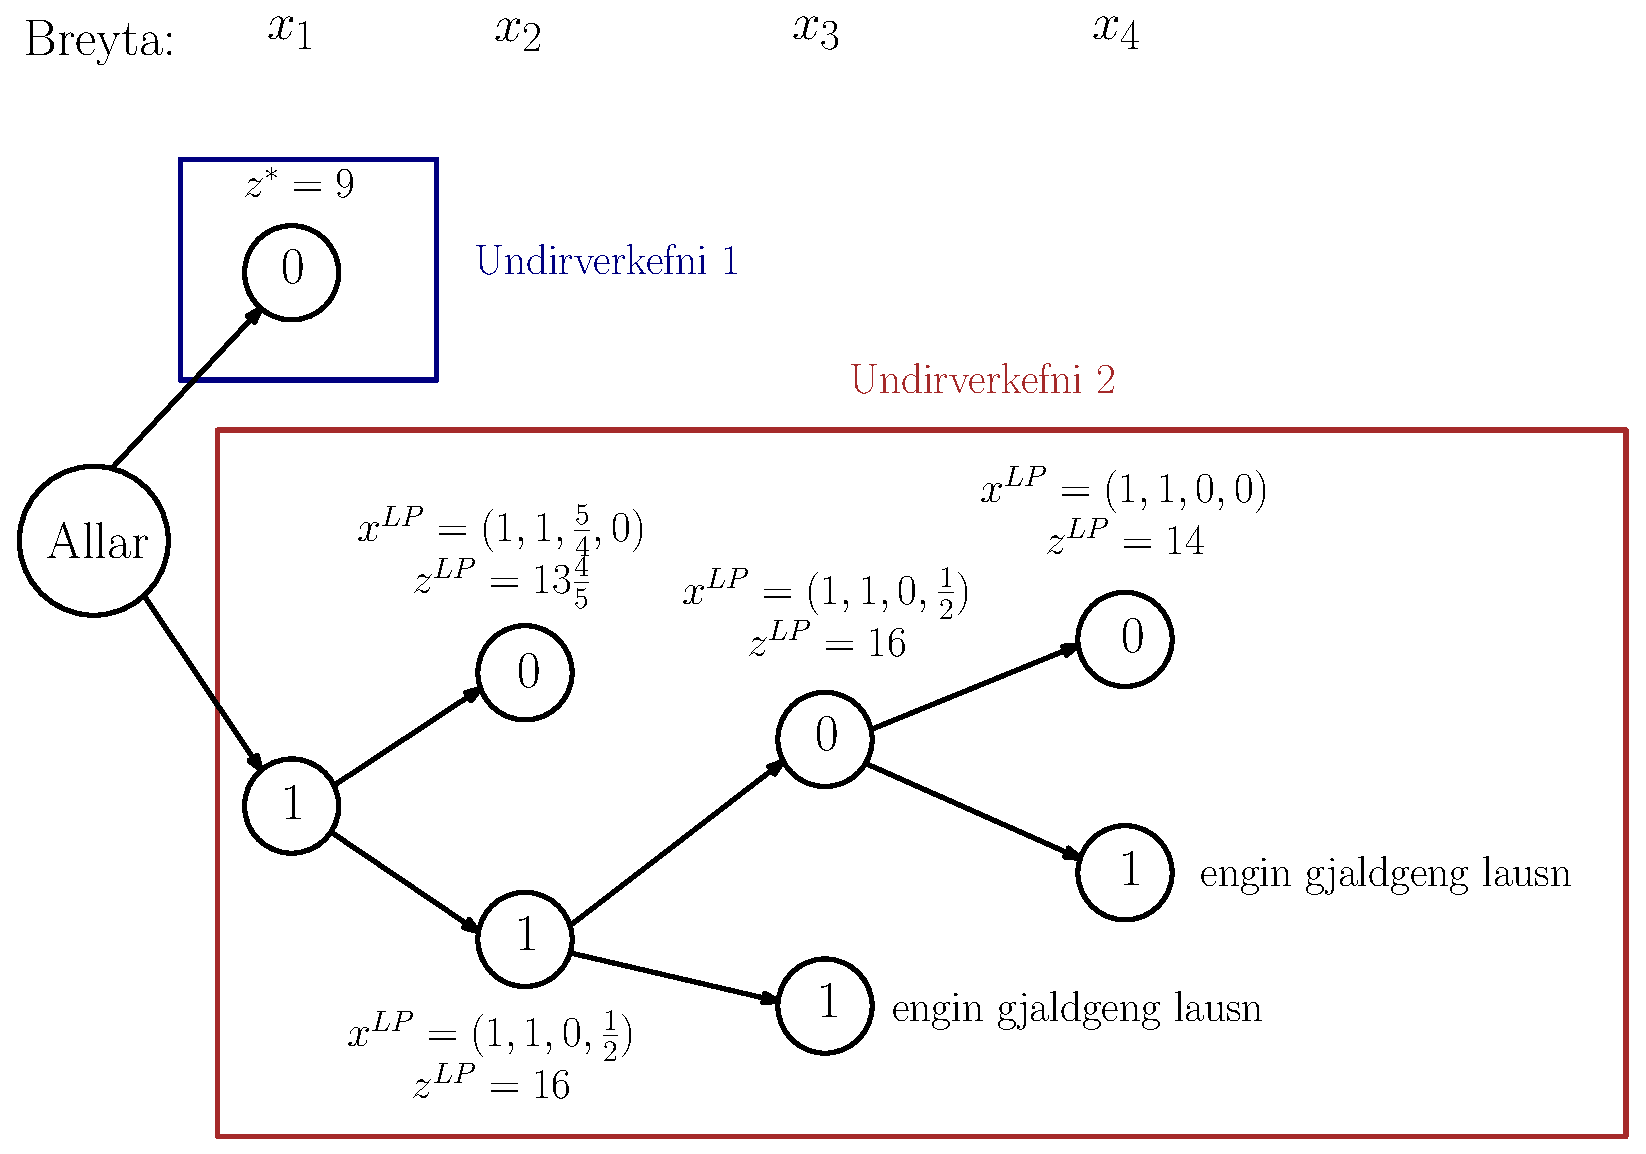
\includegraphics[width=0.9\columnwidth]{figs/branchandbound_full.eps}
\end{center}
\end{lausnSYND}

\begin{lausnSYND}[\emph{Branch-and-bound} með \textsc{glpk}] Þó svo \textsc{glpk} geti leyst tvíkostaverkefni, sbr. \texttt{var x, binary;} þá er minnsta mál að beita LP-tilslökun, og bæta við einni og einni skorðu fyrir hvert undirverkefni eins og gert var hér að ofan. Hér skiptir mestu máli að vera skipulagður í uppsetningu og kommenta réttar línur í hvert sinn forritið er keyrt.
\lstinputlisting{../glpk/branchandbound.mod}
  
\end{lausnSYND}


\subsection{\emph{Branch and bound} fyrir MIP}
\emph{Branch and bound} fyrir blönduð heiltöluverkefni.
\begin{daemi}
$$ \max_{\vec{x}} z = 4 x_1 - 2  x_2 + 7 x_3 - x_4$$
m.t.t. sk. 
\[\begin{array}{rrrrcl}
  x_1 &        &+~ 5 x_3 &        & \le & 10 \\
  x_1 &+~x_2   &-~   x_3 &        & \le & 1 \\
 6x_1 &-~ 5x_2 &         &        & \le & 0 \\
 -x_1 &        &+~  2x_3 & -~2x_4 & \le & 3
\end{array}\]
og
\begin{eqnarray*}
x_j \geq 0&& \mbox{ $j=1,2,3,4$. }\\
x_j && \mbox{ heiltala, $j=1,2,3$. }\\
x_4 &&  \mbox{ samfelld.}
\end{eqnarray*}
\end{daemi}



\begin{lausn}\hspace{.1cm}
  \begin{enumerate}[label=(\arabic{*})]\setcounter{enumi}{-1}
    \item Köllum fyrsta undirverkefnið $\mathcal{U}_0$. Setjum $z^*=-\infty$ (besta þekkta lausn á MIP hingað til).    
    Leysum línl. bestunarverkefnið með því að slaka á heiltölu kröfunni í $\mathcal{U}_0$.
 \begin{samepage}   \begin{aths} Annaðhvort í höndunum (Simplex-tafla) eða með \textsc{glpk}.     \end{aths}\end{samepage}
    Fáum LP-lausn: $\vec{x}=(1.25,1.5,1.75,0)$ með $z=14.25$.

    Sjáum að $x_1,x_2$ og $x_3$ eru ekki heiltölur, og þurfum því að kvísla verkefninu í frekari undirverkefni.

    Efra mark er $14.25$ -- við nálgum ekki því $x_4$ er \emph{ekki} heiltölubreyta.

    \item Veljum $x_1=1.25$ til að kvísla eftir:
    
    \begin{tabular}{p{7cm}|p{5cm}}
      $\mathcal{U}_0$ ásamt \mbox{$\mathcal{U}_1:~x_1\leq1$} &  $\mathcal{U}_0$ ásamt \mbox{$\mathcal{U}_2:~x_1\geq2$} \\
      \mbox{$\Rightarrow$ $\vec{x}=(1,1.2,1.8,0)$ með $z=14.2$}. &
      \mbox{$\Rightarrow$ engin gjaldgeng lausn}.
    \end{tabular}
    
    \item Getum eytt $\mathcal{U}_2$. Kvíslum $\mathcal{U}_1$ eftir $x_2=1.2$

    \begin{tabular}{p{6cm}|p{6cm}}
      $\mathcal{U}_0,\mathcal{U}_1$ ásamt \mbox{$\mathcal{U}_3:~x_2\leq1$} &
      $\mathcal{U}_0,\mathcal{U}_1$ ásamt \mbox{$\mathcal{U}_4:~x_2\leq2$} \\
      $\Rightarrow$ $\vec{x}=({\color{red}{0.833}},1,1.833,0)$ með $z=14.1667$. &
      $\Rightarrow$ $\vec{x}=({\color{red}{0.833}},2,1.833,0)$ með $z=12.1667$. 
    \end{tabular}

    \item Getum ekki eytt, en kvíslum frekar $\mathcal{U}_3$ því það hefur hærra efra mark. Bíðum með $\mathcal{U}_4$.
    Kvíslum $\mathcal{U}_3$  eftir $x_1=0.833$:

    \begin{tabular}{p{6cm}|p{6cm}}
      $\mathcal{U}_0,\mathcal{U}_1,\mathcal{U}_3$ ásamt \mbox{$\mathcal{U}_5:~x_1\leq0$} &
      $\mathcal{U}_0,\mathcal{U}_1,\mathcal{U}_3$ ásamt \mbox{$\mathcal{U}_6:~x_1\leq1$} \\
      $\Rightarrow$ engin gjaldgeng lausn &
      $\Rightarrow$ $\vec{x}=(0,0,2,0.5)$ með $z=13.5$. \\
      $\Rightarrow$ eyðum! &
      Fundum löglega lausn á $\mathcal{U}_0$, svo við uppfærum $z^*=13.5$. \\
      & $\Rightarrow$ eyðum! 
    \end{tabular}

    \item
    Getum núna eytt $\mathcal{U}_4$ því efra mark þess er $12.667<z^*$.
  
    \item Höfum afgreitt öll undirverkefni. Besta lausn er því $\vec{x}^*=(0,0,2,0.5)$ með $z^*=13.5$. 
  \end{enumerate}

\end{lausn}






\subsection{Samantekt á \emph{Branch and Bound} fyrir IP}

\begin{itemize}
\item Upphafsskref: Lát $Z=-\infty$. \begin{aths}Athugið \emph{fathoming test}, ef ekki er hægt að eyða verkefni, þá er þetta fyrsta undirverkefni.\end{aths}
\item \ath{Kvíslun} (e. branch): Af þeim undirvandamálum sem ekki hefur verið eytt, veljið það sem síðast var búið til, eða það sem hefur besta efra mark. Skiptið upp með því að setja gildi (0 eða 1) eða með því að setja bil $x_j\le[x_j^*]$ og $x_j\ge [x_j^*]+1$ ($x_j^*$ lausn á LP-tilslökunina).
 
% translate and add:
%  typical rules are the best bound rule which greedily uses the
%  remaining subset Ri with minimal value f0(Ri), and the newest
%  bound rule which partitions the most recently created subset.
%  A common method is to use the newest bound rule (depth first
%  tree search, so we find an incumbent quickly) but when there
%  is a choice of newly created sets, to use the best bound rule
%  to choose among them.
\item \ath{Efra mark} (e. bound ): Búið til efra mark með því að leysa aflappaða vandamálið með simplex aðferðinni.
\item \ath{Eyðing} (e. fathom ): Undirvandamáli er eytt ef:
\begin{itemize}
\item $F(1)$: eframark $\le z^*$,
\item $F(2)$: afslappaða verkefni þess hefur engar leyfilegar lausnir,
\item $F(3)$: afslappaða verkefni þess hefur heiltölulausn. Þessi er ný \emph{incumbent} lausn ef hún er betri.
\end{itemize}
\item Besta lausn fundin? Halda áfram uns engin undirvandamál eru eftir.  Síðasta \emph{incumbent} lausnin er besta lausn.
\end{itemize}

\begin{comment}
\begin{daemi}[MIP (sjá bls. 518 í bók)]
$$\max_{\vec{x}} Z = 4x_1 -2 x_2 + 7 x_3 - x_4$$
m.t.t. sk.
\begin{eqnarray*}
x_1 + 5 x_3  \le  10 \\
x_1 + x_2 - x_3  \le  1 \\
6 x_1 - 5 x_2  \le  0  \\
-x_1 + 2 x_3 - 2x_4  \le  3 \\
x_j\ge 0 \mbox{ og $j=1,2,3$ eru heiltölur.}
\end{eqnarray*}
\end{daemi}
\begin{lausn}\hspace{.1cm}
\lstinputlisting{matlab/branchandbound_script.m}
\end{lausn}
\end{comment}

\section{Kvíslisnið fyrir BIP verkefni}
\ath{Kvíslisnið} (e. branch-and-cut) fyrir tvíkostaverkefni, þ.e. ákvarðanabreytur eru annaðhvort 0 eða 1.

\emph{Hugmynd}: Forvinna BIP verkefnið þannig að það taki skemmri tíma til að leysa (án þess að útiloka gjaldgenga lausn). Aðferðir flokkast undir:

\begin{description}
\item[Festa ákvörðunarbreytur] annaðhvort sem $0$ eða $1$ þannig að besta lausnin sé ekki útilokuð, t.d. ef $3 x_1 \le 2$ þá er $x_1=0$.
\item[Eyða óþarfa skorðum] sem dæmi er skorðan $3x_1+2x_2 \le 6$ ofaukið, vegna þess að $3(1)+2(1) = 5  \le 6$. Getum eytt því skorðan verður alltaf uppfyllt.
\item[Þrengja skorður] minnka gjaldgengt svæði fyrir afslappað verkefni (LP-tilslökun) án þess að útiloka gjaldgengar lausnir á BIP verkefni. 
\end{description}

\subsection{Mynda kvíslisnið}
\begin{enumerate}
\item Athuga skorður sem eru aðeins með jákvæða stuðla og $\le$
  form, $$6x_1 + 3x_2+5x_3+2x_4 \le 10$$
\item Finna hóp af breytum (minnsta þekjugrúpa) þannig að:
\begin{itemize}
\item skorðan sé ekki gjaldgeng ef allar breytur í þekjugrúpu eru
  $1$ og allar aðrar breytur eru $0$, t.d. minnsta þekjugrúpa
  $\{x_1,x_3\}$, $$6(1)+3(0)+5(1)+2(0) = 11 \not\le 10$$
\item skorðan verður gjaldgeng ef ein breyta (eða fleiri) verður $0$
  í stað $1$, t.d.   $$6(1)+3(0)+5(\mathbf{0})+2(0) = 6 \le
  10$$ eða  $$6(\mathbf{0})+3(0)+5(1)+2(0) = 5 \le 10.$$
\item Lát $N$ vera fjölda breyta í minnstu þekjugrúpu $\mathcal{G}$, þá er
  hægt að mynda kvíslisnið á eftirfarandi formi:
$$\sum_{i\in\mathcal{G}}x_i \le N - 1$$
\end{itemize}
\end{enumerate}
\begin{daemi}Kvíslisnið fyrir $$6x_1 + 3x_2+5x_3+2x_4 \le 10$$\end{daemi}
\begin{lausn}
$$x_1 + x_3 \le 1$$
og
$$x_1+x_2+x_4\le 2$$
\end{lausn}
\subsection{Reiknirit til að þrengja skorður}
\lstinputlisting{../matlab/tighten.m}
\begin{daemi}$$\max_{\vec{x}} z = 3x_1 + 2 x_2$$
m.t.t. sk.
\begin{eqnarray*}
2x_1 + 3x_2  \le  4 \\
0\le x_1\le 1, 0\le x_2 \le 1
\end{eqnarray*}
\end{daemi}
\begin{lausn}Notum reikniritið hér að ofan:
\begin{lstlisting}
>> [a,b] = tighten([2 3], 4)

a =

     1     1

b =

     1
\end{lstlisting}
Skiptum því $2x_1 + 3x_2  \le  4$ út fyrir $x_1+x_2 \le 1$.

\begin{aths}Skorðan $x_1+x_2 \le 1$ hefur minnkað lausnarsvæði línulegu-tilslökunar umtalsvert, en sker ekki burt neinar gjaldgengar lausnir á tvíkostaverkefninu. Nú vill reyndar svo til að LP lausnin er $(0,1)$. 
\end{aths}

\end{lausn}

Þrenging á skorðum er dæmi um hvernig þrengja má lausnarsvæði LP-tilslökunar með því að útbúa \ath{skurðplön} (e. cutting plane). Sjá nánar bls. 514--515.

